\begin{activity} \label{A:11.1.10} 
  \ba
  \item Let $f(x,y) = 100 - x^2-y^2$ be
  defined on the rectangular domain $R = [0,6] \times
  [1,5]$. We will approximate the double integral
  $\iint_Rf(x,y)~dA$ by a Riemann sum with $m=3$ and $n=2$.

  \begin{itemize}
  \item Figure \ref{F:11.1.activity.rectangle} shows the rectangle
    $R$.  On the figure, divide the horizontal interval $m=3$ times
    and the vertical interval $n=2$ times.

    \begin{figure}[ht]
      \begin{center}
        \includegraphics{figures/fig_11_1_activity_rectangle}
      \end{center}
      \caption{The rectangle $R$.}
      \label{F:11.1.activity.rectangle}
    \end{figure}
  \item What are the dimensions $\Delta x$ and $\Delta y$ of each
    subrectangle?  What is the area $\Delta A$ of each subrectangle? 
  \item In this activity, we will choose $(x_i^*, y_j^*)$ to be the
    lower left point in each subrectangle.  Indicate these points on
    the figure and state their coordinates.
  \item Approximate the integral $\iint_Rf(x,y)~dA$ by
    evaluating the Riemann sum
    $$
    \sum_{j=1}^n\sum_{i=1}^m f(x_i^*, y_j^*)\Delta A.
    $$
  \end{itemize}

  \item Shown in Table \ref{T:11.1.activity.1} are values for the
    function $g(x,y)$. 
    If $R=[1,3]\times[2,3]$, approximate the integral
    $\iint_Rg(x,y)~dA$ using the subdivision given by $m=4$ and
    $n=2$ and choosing the points $(x_i^*,y_j^*)$ to be the upper
    right corner of the subrectangle.

    \begin{table}
      \begin{center}
        \begin{tabular}{|c||c|c|c|c|c|c|c|c|c|}
          \hline
          $x\backslash y$ &1.00&1.25&1.50&1.75&2.00&2.25&2.50&2.75&3.00\\
          \hline
          \hline
          1.00&0.50&0.62&0.75&0.88&1.00&1.12&1.25&1.37&1.50\\
          \hline
          1.25&0.62&0.78&0.94&1.09&1.25&1.41&1.56&1.72&1.87\\
          \hline
          1.50&0.75&0.94&1.12&1.31&1.50&1.69&1.87&2.06&2.25\\
          \hline
          1.75&0.88&1.09&1.31&1.53&1.75&1.97&2.19&2.41&2.62\\
          \hline
          2.00&1.00&1.25&1.50&1.75&2.00&2.25&2.50&2.75&3.00\\
          \hline
          2.25&1.12&1.41&1.69&1.97&2.25&2.53&2.81&3.09&3.37\\
          \hline
          2.50&1.25&1.56&1.87&2.19&2.50&2.81&3.12&3.44&3.75\\
          \hline
          2.75&1.37&1.72&2.06&2.41&2.75&3.09&3.44&3.78&4.12\\
          \hline
          3.00&1.50&1.87&2.25&2.62&3.00&3.37&3.75&4.12&4.50\\
          \hline
        \end{tabular}
        \caption{Values for $g(x,y)$.}
        \label{T:11.1.activity.1}
      \end{center}
    \end{table}

  \item Shown in Figure \ref{F:11.1.activity.contour} is the contour
    map of a function $h(x,y)$.  Approximate the definite integral
    $\iint_Rf(x,y)~dA$, where $R=[-1,3]\times[-2,1]$, using a
    Riemann sum defined by $m=4$ 
    horizontal subdivisions and $n=3$ vertical subdivisions.  In each
    subrectangle, choose $(x_i^*, y_J^*)$ to be the center point,
    which we call the midpoint.

      \begin{figure}[ht]
        \begin{center}
          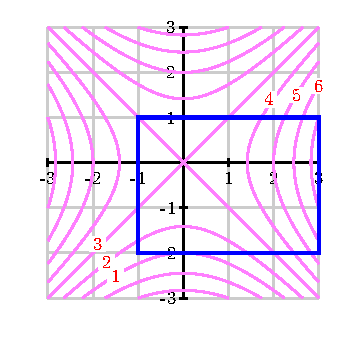
\includegraphics{figures/fig_11_1_activity_contour.eps}
        \end{center}
        \caption{Some contours of the function $h(x,y)$.}
        \label{F:11.1.activity.contour}
      \end{figure}
    \ea


\end{activity}
\aftera
